% ============================================================
% Question Bank: ch09-06 Finding Probabilities of Compound Events
% Topic Title: Finding Probabilities of Compound Events
% CCSS: 7.SP.C.8
% Questions: 30 (18 MC + 7 SA + 5 Graphical)
% ============================================================

% --- Multiple Choice Questions (18) ---

\begin{practiceQuestion}{9-6-q01}{mc}
\begin{questionText}
What is the probability of flipping two coins and getting heads on both?
\end{questionText}
\choiceA{$\frac{1}{2}$}
\choiceB{$\frac{1}{3}$}
\choiceC{$\frac{1}{4}$}
\choiceD{$\frac{3}{4}$}
\correctAnswer{C}
\explanation{Sample space: HH, HT, TH, TT ($4$ outcomes). Only HH is heads-heads. $P = \frac{1}{4}$.}
\end{practiceQuestion}

\begin{practiceQuestion}{9-6-q02}{mc}
\begin{questionText}
Two dice are rolled. What is the probability of getting a sum of $7$?
\end{questionText}
\choiceA{$\frac{1}{12}$}
\choiceB{$\frac{7}{36}$}
\choiceC{$\frac{1}{6}$}
\choiceD{$\frac{5}{36}$}
\correctAnswer{C}
\explanation{Favorable outcomes: $(1,6), (2,5), (3,4), (4,3), (5,2), (6,1)$ — that is $6$ out of $36$. $P = \frac{6}{36} = \frac{1}{6}$.}
\end{practiceQuestion}

\begin{practiceQuestion}{9-6-q03}{mc}
\begin{questionText}
A coin is flipped and a die is rolled. What is the probability of getting tails and an even number?
\end{questionText}
\choiceA{$\frac{1}{12}$}
\choiceB{$\frac{1}{6}$}
\choiceC{$\frac{1}{4}$}
\choiceD{$\frac{1}{2}$}
\correctAnswer{C}
\explanation{$P(\text{tails}) = \frac{1}{2}$ and $P(\text{even}) = \frac{3}{6} = \frac{1}{2}$. $P = \frac{1}{2} \times \frac{1}{2} = \frac{1}{4}$. Or: $3$ favorable out of $12$ total outcomes.}
\end{practiceQuestion}

\begin{practiceQuestion}{9-6-q04}{mc}
\begin{questionText}
Two dice are rolled. What is the probability of getting a sum of $2$?
\end{questionText}
\choiceA{$\frac{1}{6}$}
\choiceB{$\frac{1}{12}$}
\choiceC{$\frac{1}{36}$}
\choiceD{$\frac{2}{36}$}
\correctAnswer{C}
\explanation{The only way to get a sum of $2$ is $(1,1)$. $P = \frac{1}{36}$.}
\end{practiceQuestion}

\begin{practiceQuestion}{9-6-q05}{mc}
\begin{questionText}
A spinner has $3$ equal sections (A, B, C) and a coin is flipped. What is the probability of landing on B and getting heads?
\end{questionText}
\choiceA{$\frac{1}{2}$}
\choiceB{$\frac{1}{3}$}
\choiceC{$\frac{1}{6}$}
\choiceD{$\frac{2}{3}$}
\correctAnswer{C}
\explanation{$P(B) = \frac{1}{3}$, $P(\text{heads}) = \frac{1}{2}$. $P = \frac{1}{3} \times \frac{1}{2} = \frac{1}{6}$.}
\end{practiceQuestion}

\begin{practiceQuestion}{9-6-q06}{mc}
\begin{questionText}
Two dice are rolled. What is the probability that both dice show the same number (doubles)?
\end{questionText}
\choiceA{$\frac{1}{36}$}
\choiceB{$\frac{1}{12}$}
\choiceC{$\frac{1}{6}$}
\choiceD{$\frac{1}{3}$}
\correctAnswer{C}
\explanation{Doubles: $(1,1), (2,2), (3,3), (4,4), (5,5), (6,6)$ — that is $6$ out of $36$. $P = \frac{6}{36} = \frac{1}{6}$.}
\end{practiceQuestion}

\begin{practiceQuestion}{9-6-q07}{mc}
\begin{questionText}
Three coins are flipped. What is the probability of getting exactly $2$ heads?
\end{questionText}
\choiceA{$\frac{1}{8}$}
\choiceB{$\frac{2}{8}$}
\choiceC{$\frac{3}{8}$}
\choiceD{$\frac{4}{8}$}
\correctAnswer{C}
\explanation{Outcomes with exactly $2$ heads: HHT, HTH, THH — that is $3$ out of $8$. $P = \frac{3}{8}$.}
\end{practiceQuestion}

\begin{practiceQuestion}{9-6-q08}{mc}
\begin{questionText}
Two dice are rolled. What is the probability of getting a sum greater than $10$?
\end{questionText}
\choiceA{$\frac{1}{36}$}
\choiceB{$\frac{2}{36}$}
\choiceC{$\frac{3}{36}$}
\choiceD{$\frac{6}{36}$}
\correctAnswer{C}
\explanation{Sums greater than $10$: $11$ and $12$. Sum $11$: $(5,6), (6,5)$. Sum $12$: $(6,6)$. Total: $3$ out of $36$. $P = \frac{3}{36} = \frac{1}{12}$.}
\end{practiceQuestion}

\begin{practiceQuestion}{9-6-q09}{mc}
\begin{questionText}
A bag has $3$ red and $2$ blue marbles. You draw one marble, replace it, and draw again. What is the probability that both are red?
\end{questionText}
\choiceA{$\frac{6}{25}$}
\choiceB{$\frac{9}{25}$}
\choiceC{$\frac{3}{10}$}
\choiceD{$\frac{6}{20}$}
\correctAnswer{B}
\explanation{With replacement: $P = \frac{3}{5} \times \frac{3}{5} = \frac{9}{25}$.}
\end{practiceQuestion}

\begin{practiceQuestion}{9-6-q10}{mc}
\begin{questionText}
A coin is flipped $3$ times. What is the probability of getting all tails?
\end{questionText}
\choiceA{$\frac{1}{2}$}
\choiceB{$\frac{1}{4}$}
\choiceC{$\frac{1}{8}$}
\choiceD{$\frac{3}{8}$}
\correctAnswer{C}
\explanation{$P = \frac{1}{2} \times \frac{1}{2} \times \frac{1}{2} = \frac{1}{8}$. Or: $1$ favorable (TTT) out of $8$ total outcomes.}
\end{practiceQuestion}

\begin{practiceQuestion}{9-6-q11}{mc}
\begin{questionText}
Two dice are rolled. What is the probability that the sum is even?
\end{questionText}
\choiceA{$\frac{1}{4}$}
\choiceB{$\frac{1}{3}$}
\choiceC{$\frac{1}{2}$}
\choiceD{$\frac{2}{3}$}
\correctAnswer{C}
\explanation{Even sums occur when both dice are even or both are odd. Both even: $3 \times 3 = 9$. Both odd: $3 \times 3 = 9$. Total: $18$ out of $36$. $P = \frac{18}{36} = \frac{1}{2}$.}
\end{practiceQuestion}

\begin{practiceQuestion}{9-6-q12}{mc}
\begin{questionText}
A spinner has $4$ equal sections ($1, 2, 3, 4$) and a die is rolled. What is the probability that both show a $3$?
\end{questionText}
\choiceA{$\frac{1}{10}$}
\choiceB{$\frac{1}{24}$}
\choiceC{$\frac{2}{10}$}
\choiceD{$\frac{1}{4}$}
\correctAnswer{B}
\explanation{$P(\text{spinner} = 3) = \frac{1}{4}$, $P(\text{die} = 3) = \frac{1}{6}$. $P = \frac{1}{4} \times \frac{1}{6} = \frac{1}{24}$.}
\end{practiceQuestion}

\begin{practiceQuestion}{9-6-q13}{mc}
\begin{questionText}
Two coins are flipped. What is the probability of getting at least one head?
\end{questionText}
\choiceA{$\frac{1}{4}$}
\choiceB{$\frac{1}{2}$}
\choiceC{$\frac{3}{4}$}
\choiceD{$1$}
\correctAnswer{C}
\explanation{At least one head: HH, HT, TH — that is $3$ out of $4$. $P = \frac{3}{4}$. Or: $1 - P(\text{no heads}) = 1 - \frac{1}{4} = \frac{3}{4}$.}
\end{practiceQuestion}

\begin{practiceQuestion}{9-6-q14}{mc}
\begin{questionText}
A bag has $4$ green and $6$ yellow marbles. You pick one marble without replacement and then pick another. What is the probability that the first is green and the second is yellow?
\end{questionText}
\choiceA{$\frac{24}{100}$}
\choiceB{$\frac{24}{90}$}
\choiceC{$\frac{4}{15}$}
\choiceD{$\frac{6}{10}$}
\correctAnswer{C}
\explanation{$P(\text{green first}) = \frac{4}{10}$. After removing a green, $P(\text{yellow second}) = \frac{6}{9}$. $P = \frac{4}{10} \times \frac{6}{9} = \frac{24}{90} = \frac{4}{15}$.}
\end{practiceQuestion}

\begin{practiceQuestion}{9-6-q15}{mc}
\begin{questionText}
Two dice are rolled. What is the probability that the product (not the sum) of the two numbers is $12$?
\end{questionText}
\choiceA{$\frac{2}{36}$}
\choiceB{$\frac{4}{36}$}
\choiceC{$\frac{3}{36}$}
\choiceD{$\frac{6}{36}$}
\correctAnswer{B}
\explanation{Pairs with product $12$: $(2,6), (6,2), (3,4), (4,3)$ — that is $4$ out of $36$. $P = \frac{4}{36} = \frac{1}{9}$.}
\end{practiceQuestion}

\begin{practiceQuestion}{9-6-q16}{mc}
\begin{questionText}
A coin is flipped and a die is rolled. What is the probability of getting heads and a number greater than $4$?
\end{questionText}
\choiceA{$\frac{1}{12}$}
\choiceB{$\frac{1}{6}$}
\choiceC{$\frac{2}{12}$}
\choiceD{$\frac{1}{3}$}
\correctAnswer{B}
\explanation{$P(\text{heads}) = \frac{1}{2}$. Numbers greater than $4$: $5, 6$, so $P = \frac{2}{6} = \frac{1}{3}$. $P = \frac{1}{2} \times \frac{1}{3} = \frac{1}{6}$.}
\end{practiceQuestion}

\begin{practiceQuestion}{9-6-q17}{mc}
\begin{questionText}
Two spinners are spun. Spinner 1 has sections $\{1, 2, 3\}$ and Spinner 2 has sections $\{A, B\}$. What is the probability of getting $2$ and $A$?
\end{questionText}
\choiceA{$\frac{1}{3}$}
\choiceB{$\frac{1}{5}$}
\choiceC{$\frac{1}{6}$}
\choiceD{$\frac{2}{6}$}
\correctAnswer{C}
\explanation{$P(2) = \frac{1}{3}$, $P(A) = \frac{1}{2}$. $P = \frac{1}{3} \times \frac{1}{2} = \frac{1}{6}$.}
\end{practiceQuestion}

\begin{practiceQuestion}{9-6-q18}{mc}
\begin{questionText}
Three coins are flipped. What is the probability of getting NO heads (all tails)?
\end{questionText}
\choiceA{$\frac{1}{2}$}
\choiceB{$\frac{1}{4}$}
\choiceC{$\frac{1}{8}$}
\choiceD{$\frac{3}{8}$}
\correctAnswer{C}
\explanation{Only one outcome out of $8$ is all tails (TTT). $P = \frac{1}{8}$.}
\end{practiceQuestion}

% --- Short Answer Questions (7) ---

\begin{practiceQuestion}{9-6-q19}{sa}
\begin{questionText}
Two dice are rolled. What is the probability that the sum is $10$ or greater? Write your answer as a fraction in simplest form.
\end{questionText}
\correctAnswer{$\frac{1}{6}$}
\explanation{Sum $10$: $(4,6), (5,5), (6,4)$ — $3$ outcomes. Sum $11$: $(5,6), (6,5)$ — $2$. Sum $12$: $(6,6)$ — $1$. Total: $6$ out of $36$. $P = \frac{6}{36} = \frac{1}{6}$.}
\end{practiceQuestion}

\begin{practiceQuestion}{9-6-q20}{sa}
\begin{questionText}
A coin is flipped and a die is rolled. What is the probability of getting tails and a $1$? Write your answer as a fraction.
\end{questionText}
\correctAnswer{$\frac{1}{12}$}
\explanation{$P(\text{tails}) = \frac{1}{2}$, $P(1) = \frac{1}{6}$. $P = \frac{1}{2} \times \frac{1}{6} = \frac{1}{12}$.}
\end{practiceQuestion}

\begin{practiceQuestion}{9-6-q21}{sa}
\begin{questionText}
A bag has $5$ red and $5$ blue marbles. You draw two marbles without replacement. What is the probability that both are blue? Write your answer as a fraction in simplest form.
\end{questionText}
\correctAnswer{$\frac{2}{9}$}
\explanation{$P(\text{first blue}) = \frac{5}{10}$. $P(\text{second blue}) = \frac{4}{9}$. $P = \frac{5}{10} \times \frac{4}{9} = \frac{20}{90} = \frac{2}{9}$.}
\end{practiceQuestion}

\begin{practiceQuestion}{9-6-q22}{sa}
\begin{questionText}
Two dice are rolled. What is the probability that the sum is exactly $6$? Write your answer as a fraction in simplest form.
\end{questionText}
\correctAnswer{$\frac{5}{36}$}
\explanation{Outcomes with sum $6$: $(1,5), (2,4), (3,3), (4,2), (5,1)$ — $5$ out of $36$. $P = \frac{5}{36}$.}
\end{practiceQuestion}

\begin{practiceQuestion}{9-6-q23}{sa}
\begin{questionText}
A spinner has $4$ equal sections (W, X, Y, Z). It is spun twice. What is the probability of getting the same letter both times? Write your answer as a fraction in simplest form.
\end{questionText}
\correctAnswer{$\frac{1}{4}$}
\explanation{Matching pairs: (W,W), (X,X), (Y,Y), (Z,Z) — $4$ out of $16$. $P = \frac{4}{16} = \frac{1}{4}$.}
\end{practiceQuestion}

\begin{practiceQuestion}{9-6-q24}{sa}
\begin{questionText}
A bag has $2$ red, $3$ blue, and $5$ green marbles. You draw one marble, replace it, and draw again. What is the probability that both marbles are green? Write your answer as a fraction in simplest form.
\end{questionText}
\correctAnswer{$\frac{1}{4}$}
\explanation{$P(\text{green}) = \frac{5}{10} = \frac{1}{2}$. With replacement: $P = \frac{1}{2} \times \frac{1}{2} = \frac{1}{4}$.}
\end{practiceQuestion}

\begin{practiceQuestion}{9-6-q25}{sa}
\begin{questionText}
Three coins are flipped. What is the probability of getting exactly $1$ head? Write your answer as a fraction in simplest form.
\end{questionText}
\correctAnswer{$\frac{3}{8}$}
\explanation{Outcomes with exactly $1$ head: HTT, THT, TTH — that is $3$ out of $8$. $P = \frac{3}{8}$.}
\end{practiceQuestion}

% --- Graphical Questions (3 GMC + 2 GSA) ---

\begin{practiceQuestion}{9-6-q26}{gmc}
\begin{questionText}
The table shows all possible sums when two dice are rolled. What is the probability of rolling a sum of $8$?

\begin{center}
\begin{tabular}{|c|c|c|c|c|c|c|}
\hline
$+$ & \textbf{1} & \textbf{2} & \textbf{3} & \textbf{4} & \textbf{5} & \textbf{6} \\
\hline
\textbf{1} & $2$ & $3$ & $4$ & $5$ & $6$ & $7$ \\
\hline
\textbf{2} & $3$ & $4$ & $5$ & $6$ & $7$ & \cellcolor{funBlue!20}$8$ \\
\hline
\textbf{3} & $4$ & $5$ & $6$ & $7$ & \cellcolor{funBlue!20}$8$ & $9$ \\
\hline
\textbf{4} & $5$ & $6$ & $7$ & \cellcolor{funBlue!20}$8$ & $9$ & $10$ \\
\hline
\textbf{5} & $6$ & $7$ & \cellcolor{funBlue!20}$8$ & $9$ & $10$ & $11$ \\
\hline
\textbf{6} & $7$ & \cellcolor{funBlue!20}$8$ & $9$ & $10$ & $11$ & $12$ \\
\hline
\end{tabular}
\end{center}
\end{questionText}
\choiceA{$\frac{4}{36}$}
\choiceB{$\frac{5}{36}$}
\choiceC{$\frac{6}{36}$}
\choiceD{$\frac{8}{36}$}
\correctAnswer{B}
\explanation{Outcomes with sum $8$: $(2,6), (3,5), (4,4), (5,3), (6,2)$ — that is $5$. $P = \frac{5}{36}$.}
\end{practiceQuestion}

\begin{practiceQuestion}{9-6-q27}{gmc}
\begin{questionText}
The tree diagram shows the outcomes for flipping two coins. What is the probability of getting at least one tail?

\begin{center}
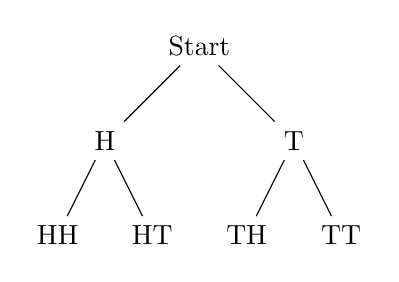
\begin{tikzpicture}[scale=0.8,
  level 1/.style={sibling distance=3cm, level distance=1.5cm},
  level 2/.style={sibling distance=1.5cm, level distance=1.5cm}]
  \node {Start}
    child {node {H}
      child {node {HH}}
      child {node {HT}}
    }
    child {node {T}
      child {node {TH}}
      child {node {TT}}
    };
\end{tikzpicture}
\end{center}
\end{questionText}
\choiceA{$\frac{1}{4}$}
\choiceB{$\frac{1}{2}$}
\choiceC{$\frac{3}{4}$}
\choiceD{$\frac{2}{4}$}
\correctAnswer{C}
\explanation{Outcomes with at least one tail: HT, TH, TT — that is $3$ out of $4$. $P = \frac{3}{4}$.}
\end{practiceQuestion}

\begin{practiceQuestion}{9-6-q28}{gmc}
\begin{questionText}
The table below shows the sample space for spinning two spinners. Spinner 1 has sections $\{1, 2, 3\}$ and Spinner 2 has sections $\{A, B\}$. If each outcome is equally likely, what is the probability of getting an odd number and the letter B?

\begin{center}
\begin{tabular}{|c|c|c|}
\hline
 & \textbf{A} & \textbf{B} \\
\hline
\textbf{1} & $(1,A)$ & \cellcolor{funGreen!20}$(1,B)$ \\
\hline
\textbf{2} & $(2,A)$ & $(2,B)$ \\
\hline
\textbf{3} & $(3,A)$ & \cellcolor{funGreen!20}$(3,B)$ \\
\hline
\end{tabular}
\end{center}
\end{questionText}
\choiceA{$\frac{1}{6}$}
\choiceB{$\frac{2}{6}$}
\choiceC{$\frac{3}{6}$}
\choiceD{$\frac{4}{6}$}
\correctAnswer{B}
\explanation{Odd numbers: $1, 3$. Favorable outcomes: $(1,B)$ and $(3,B)$ — $2$ out of $6$. $P = \frac{2}{6} = \frac{1}{3}$.}
\end{practiceQuestion}

\begin{practiceQuestion}{9-6-q29}{gsa}
\begin{questionText}
The table shows all possible products when two dice are rolled. How many outcomes give a product of $6$? Write the probability as a fraction in simplest form.

\begin{center}
\begin{tabular}{|c|c|c|c|c|c|c|}
\hline
$\times$ & \textbf{1} & \textbf{2} & \textbf{3} & \textbf{4} & \textbf{5} & \textbf{6} \\
\hline
\textbf{1} & $1$ & $2$ & $3$ & $4$ & $5$ & $6$ \\
\hline
\textbf{2} & $2$ & $4$ & $6$ & $8$ & $10$ & $12$ \\
\hline
\textbf{3} & $3$ & $6$ & $9$ & $12$ & $15$ & $18$ \\
\hline
\textbf{4} & $4$ & $8$ & $12$ & $16$ & $20$ & $24$ \\
\hline
\textbf{5} & $5$ & $10$ & $15$ & $20$ & $25$ & $30$ \\
\hline
\textbf{6} & $6$ & $12$ & $18$ & $24$ & $30$ & $36$ \\
\hline
\end{tabular}
\end{center}
\end{questionText}
\correctAnswer{$\frac{1}{9}$}
\explanation{Products of $6$: $(1,6), (2,3), (3,2), (6,1)$ — $4$ outcomes. $P = \frac{4}{36} = \frac{1}{9}$.}
\end{practiceQuestion}

\begin{practiceQuestion}{9-6-q30}{gsa}
\begin{questionText}
Look at the tree diagram for flipping three coins. What is the probability of getting exactly $2$ tails? Write your answer as a fraction in simplest form.

\begin{center}
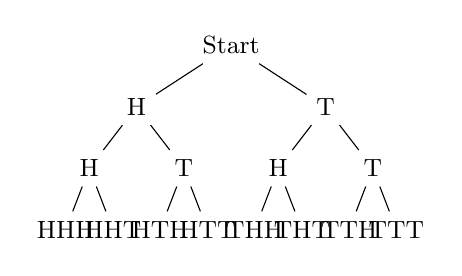
\begin{tikzpicture}[scale=0.6,
  level 1/.style={sibling distance=4cm, level distance=1.3cm},
  level 2/.style={sibling distance=2cm, level distance=1.3cm},
  level 3/.style={sibling distance=1cm, level distance=1.3cm}]
  \node {\small Start}
    child {node {\small H}
      child {node {\small H}
        child {node {\small HHH}}
        child {node {\small HHT}}
      }
      child {node {\small T}
        child {node {\small HTH}}
        child {node {\small HTT}}
      }
    }
    child {node {\small T}
      child {node {\small H}
        child {node {\small THH}}
        child {node {\small THT}}
      }
      child {node {\small T}
        child {node {\small TTH}}
        child {node {\small TTT}}
      }
    };
\end{tikzpicture}
\end{center}
\end{questionText}
\correctAnswer{$\frac{3}{8}$}
\explanation{Outcomes with exactly $2$ tails: HTT, THT, TTH — that is $3$ out of $8$. $P = \frac{3}{8}$.}
\end{practiceQuestion}
